\chapter{Introduction}
\label{ch:intro}

%Mathematical theorem provers comes equipped with libraries of formalized mathematics. 
A large library of formalized, ready-to-use mathematics has long been the pursuit of mathematicians and computer scientists.  
The influential QED manifesto~\cite{boyer1994qed}, released in 1994, envisioned a library in which all mathematics is formalized and rigorously checked. The QED manifesto believed in one-formalization-fits-all approach to building this library.
Diversity in mathematical formalizations was a big obstacle towards realizing the library described by QED. There was not an agreement even on which foundation to use for formalizing all of mathematics~\cite{qedrealoaded2016}.  Since then, mathematical knowledge management (MKM) became an active area of research framing a new vision for the large math library. The universal digital math library (UDML), described in~\cite{farmer2004mkm}, is a collection of heterogeneous, intercommunicating systems and building this library is described as a grand challenge facing MKM. 

Despite the many efforts dedicated to building math libraries\ednote{some references}, a universal large library has not become a reality. One reason is that developing and maintaining libraries of mathematics requires a lot of manpower. One would want to believe that this human effort is put into the creative work of formalizing new pieces of knowledge. By examining current libraries of theorem provers, we know this is not always the case. The process of creating libraries for theorem provers involve a lot of redundancy. We give examples from libraries of formal systems in Chapter~\ref{ch:redundancy}. To understand why this redundancy exists, we examine the formalization of \lstmath{Monoid} in algebra textbooks versus in interactive theorem provers. 

\lstmath{Monoid} is an algebraic structure that describes algebras with carrier set and associative binary operation over that set that has a unit. The definition given in~\cite{jacobson1985basic}  is 
\begin{quote}
    A monoid is a triple $(M,p,1)$ in which $M$ is a non-vacuous set, $p$ is an associative binary composition (or product) in $M$, and $1$ is an element of $M$ such that $p(1,a)= a = p(a,1)$ for all $a \in M$ 
\end{quote}
The definition of \lstmath{Monoid} is followed by the definition of its homomorphism as
\begin{quote}
If $M$ and $M^\prime$ are monoids, then a map $\eta$ of $M$ into $M^\prime$ is called a homomorphism if 
\begin{multicols}{3}
    $\eta(ab)=\eta(a)\eta(b)$, \vfill   
    \columnbreak
    $\eta(1) = 1$, \vfill   
    \columnbreak 
    $a,b \in M$  \vfill    
\end{multicols}
\end{quote}
More monoid-related constructions are defined, like submonoid, and quotient monoids. The same constructions are defined for \lstmath{Group} and \lstmath{Ring}. 
%Mathematics presented in textbooks rely on the human understanding to be able to generalize these concepts. For example, \cite{jacobson1985basic} does not provide an explicit definition for group homomorphism, but proceeds to use it. 

Formal systems\footnote{We use the term \emph{formal systems} to refer to all computer systems with logical foundations, be it automatic theorem prover (ATP), interactive theorem prover (ITP), specification system, or others.} present algebraic structures using axiomatic theories\ednote{should I define axiomatic theories?}. \lstmath{Monoid} and its homomorphism are presented axiomatically in a minimal (imaginary) computer language as follows 
\begin{lstlisting}[mathescape]
theory Monoid { 
  A : type 
  e : A
  op : A $\to$ A $\to$ A
  lunit : (x : A) $\to$ op e x = x 
  runit : (x : A) $\to$ op x e = x 
  assoc : (x y z : A) $\to$ op x (op y z) = op (op x y) z
}

theory MonoidHom { 
  M1, M2 : Monoid  
  hom : M1.A $\to$ M2.A 
  pres-e : hom (M1.e) = M2.e
  pres-op : (x y : M1.A) $\to$ hom (M1.op x y) = M2.op (hom x) (hom y) 
}
\end{lstlisting}
Let's now define \lstmath{Group} and \lstmath{Group} homomorphism within the same language
\begin{lstlisting}[mathescape]
theory Group {
  A : type 
  e : A
  op : A $\to$ A $\to$ A
  inv : A $\to$ A
  lunit_e : (x : A) $\to$ op e x = x
  runit_e : (x : A) $\to$ op x e = x
  linverse : (x : A) $\to$ op x (inv x) == e
  rinverse : (x : A) $\to$ op (inv x) x == e
  associative : (x y z : A) $\to$ op x (op y z) = op (op x y) z
}

theory GroupHom { 
  G1, G2 : Group 
  hom : G1.A $\to$ G2.A
  pres-e : hom (G1.e) = G2.e
  pres-op : (x y : G1.A) $\to$ hom (G1.op x y) = G2.op (hom x) (hom y)
  pres-inv : (x : G1.A) $\to$ hom (G1.inv x) = G2.inv (hom x)
}
\end{lstlisting}
Notice how the two definitions of homomorphisms are similar and do not depend so much on the details of the theory. Generally, the homomorphism of a theory \lstmath{X} is a mapping between two instances of \lstmath{X} and has $3$ components 1) the $2$ instances of the theory, 2) the function \lstmath{hom} that maps the carriers of the $2$ instances, and 3) preservation axioms \lstmath{pres-x} for every operation symbol \lstmath{x}. The preservation axioms follow the pattern
\begin{lstlisting}[mathescape]
hom (op$_1$ x$_1$ .. x$_n$) = op$_2$ (hom x$_1$) .. (hom x$_n$)
\end{lstlisting}
Observing this pattern gives rise to some questions
 
\begin{itemize}
\item[Q1] Is this pattern specific to \lstmath{Monoid}, \lstmath{Group}, and their homomorphisms? 
\end{itemize}    
\lstmath{Monoid} and \lstmath{Group} are two of many algebraic structures used in abstract algebra. The commonalities between these structures is the subject of study of universal algebra, and is captured by the following definition~\cite{mckenzie1987algebras}
\begin{quote}
    An algebra is an ordered pair $\langle A, F \rangle$ such that $A$ is a nonempty set and $F = \langle F_i : i \in I \rangle$ where $F_i$ is a finitary operation on $A$ for each $i \in I$. $A$ is called the universe of $\langle A, F \rangle$, $F_i$ is referred to as a fundamental or basic operation of $\langle A, F \rangle$ for each $i \in I$, and $I$ is called the index set of the set of operation symbols for $\langle A, F \rangle$. 
\end{quote}
\ednote{look for a text book that explicitly state axioms. The properties of the function symbols, which are mentioned in mathematics textbooks but not always stated, are stated as axioms in formal systems, and so we defined an algebraic theory to be a type ($\langle A, F \rangle$,$E$), where $E$ is the set of axioms.}
\todo{check the sanella software specification book for this definition. }

For every theory that fit in this definition, we have a uniform definition of homomorphism, subalgebra, quotient algebra, term language and others. 

\begin{itemize}
    \item[Q2] What meta theory is used? 
\end{itemize}
While libraries of mathematics contain many different pieces of mathematical knowledge, we choose to focus on abstract algebra. Mathematicians have already studied the commonalities in this field and created universal algebra to describe it. Hence, we have a strong meta theory to understand how the definitions relate to each other. On the other hand, the MKM community have not utilized these abstraction in library building. This is the gap we are trying to fill in this work.  

\begin{itemize}
    \item[Q3] Is there enough information that can be generated? 
\end{itemize}
There is a lot of information that can be generated for one algebraic structure.  We list X\ednote{find the number} of them in Section~\ref{sec:toBeGenerated}. There are also many algebraic structures used in mathematics and computer science. While the hierarchy the comes in mind usually is \\
\lstmath{Semigroup $\to$ Monoid $\to$ Group $\to$ Semiring $\to$ Ring}, there are many more and are structured in a more complex way, as we discuss in Chapter~\ref{ch:library}. 
The list in~\cite{jipsen} defines over $300$ structure. There are also many being used in the meta theory of programming languages, like \lstmath{Applicative} and \lstmath{Monad}. 
Algebraic software specification is another area that uses algebraic theories to describe software. The broad scope of software systems make us believe there is a lot of algebraic structures being produced by this community.  

\begin{itemize}
    \item[Q4] What abstractions are needed (barriers exists) to generate this knowledge?
\end{itemize}\todo{This question can be written in a better way}.  
\lstmath{Monoid} theory is one of those captured by this abstraction. We have given a definition of \lstmath{Monoid} in an imaginary language that fits in this abstraction. In Figure~\ref{fig:mon-diff-lang}, we show the definitions of \lstmath{Monoid} in $5$ different language. 
\begin{figure}
    \footnotesize
\begin{tabular}{p{6.3cm} p{7cm}}
\underline{Haskell}
\begin{minted}[mathescape]{haskell}
class Semigroup a => 
      Monoid a 
 where 
  mempty :: a 
  mappend :: a -> a -> a 
  mappend = (<>) 
  mconcat :: [a] -> a 
  mconcat = 
   foldr mappend mempty 
\end{minted} 
\underline{Lean}
\begin{leancode}
class monoid (M : Type u)
 extends semigroup M, 
         has_one M :=
  (one_mul : ~$\forall$~ a : M, 
           1 * a = a) 
  (mul_one : ~$\forall$~ a : M, 
           a * 1 = a)   
\end{leancode} 
% [mathescape=true, escape_inside=~~]
\underline{Coq}
\begin{minted}[mathescape=true, escapeinside=~~]{coq}
class Monoid {A : type}
 (dot : A ~$\to$~ A ~$\to$~ A)
 (one : A) : Prop := {
  dot_assoc : 
   forall x y z : A, 
   (dot x (dot y z)) = 
   dot (dot x y) z
  unit_left : forall x, 
   dot one x = x 
  unit_right : forall x, 
   dot x one = x              
}
~$\text{\textit{Alternative Definition:}}$~
Record monoid := {
 dom : Type; 
 op : dom -> dom -> dom 
  where "x * y" := op x y; 
 id : dom where "1" := id; 
 assoc : forall x y z, 
  x * (y * z) = (x * y) * z; 
 left_neutral : forall x,   
  1 * x = x; 
 right_neutal : forall x,
  x * 1 = x; 
}
\end{minted} 
&
\underline{Agda}
\begin{agdacode}
record Monoid c ~$\ell$~ : 
   Set (suc (c ~$\sqcup$~ ~$\ell$~)) where 
 infixl 7 _~$\bullet$~_
 infix 4 _~$\approx$~_
 field 
  Carrier : Set c 
  _~$\approx$~_ : Rel Carrier ~$\ell$~ 
  _~$\bullet$~_ : Op~$_2$~ Carrier 
  isMonoid : IsMonoid _~$\approx$~_ _~$\bullet$~_ ~$\varepsilon$~ 
  
record IsMonid (~$\bullet$~ : Op~$_2$~) (~$\varepsilon$~ : A) 
 : Set (a ~$\sqcup$~ ~$\ell$~) where 
  field 
   isSemiring : IsSemiring ~$\bullet$~ 
   identity : Identity ~$\varepsilon$~ 
       
   open IsSemigroup isSemigroup public 
   
   identity~$^l$~ : LeftIdentity ~$\varepsilon$~ ~$\bullet$~ 
   identity~$^l$~ = proj~$_1$~ identity 
   identity~$^r$~ : Rightdentity ~$\varepsilon$~ ~$\bullet$~ 
   identity~$^r$~ = proj~$_2$~ identity        
\end{agdacode}       
\underline{MMT}
\begin{minted}[mathescape=true, escapeinside=~~]{mmt} 
theory Semigroup : ?NatDed = 
 u : sort 
 comp : tm u ~$\to$~ tm u ~$\to$~ tm u 
  # 1 * 2 prec 40
 assoc : ~$\vdash$~ ~$\forall$~ [x, y, z]
  (x * y) * z = x * (y * z)    
 assocLeftToRight : 
  {x,y,z} ~$\vdash$~ (x * y) * z 
          = x * (y * z) 
  = [x,y,z] 
   allE (allE (allE assoc x) y) z
 assocRightToLeft : 
  {x,y,z} ~$\vdash$~  x * (y * z) 
           = (x * y) * z 
  = [x,y,z] sym assocLR 
theory Monoid : ?NatDed 
 includes ?Semigroup 
 unit : tm u # e 
 unit_axiom : ~$\vdash$~ ~$\forall$~ [x] = x * e = x       
\end{minted}      
\end{tabular}  

    \caption{Representation of \lstinline|Monoid| theory in different languages.}
    \label{fig:mon-diff-lang}
\end{figure}
Although the $5$ definitions refer to the same mathematical concept, they look very different. The reason is that every system employ different design decisions. In some cases, as in Haskell and MMT, the theory \monoid is defined as an extension of \semigroup. Despite this being useful, there is no reason why a developer might not want to add a theory \unital (a non-associative \monoid), to the hierarchy. Exposing this hierarchy to the user makes their code vulnerable in case the hierarchy changes. This problem occurred when Haskell changed the hierarchy of type classes when \lstmath{Applicative} became a superclass for \lstmath{Monad} ~\cite{wiki:haskell_hierarch}. The work in \cite{cohen2020hierarchy} discusses this problem. The two Coq definitions takes two extreme views to the bundling problem~\cite{lean2019,alhassy2019,spitters2011type} by either having the carrier and all the function symbols as arguments (the first definition) or having all elements of the theory as declarations of a record type (the second definition). 
The formalization of the Algebraic hierarchy in the Agda standard library is based on setoids (sets equipped with the equivalence relation). Therefore, we find an extra field of the definition of \monoid corresponding to the equivalence relation $\_\approx\_$. 

Not only are library definitions diverse, but so are user projects. When design decisions are embedded that much into the definitions of the library, users find it difficult to reuse it in their projects and are forced to redefine many pieces. That leads to many libraries formalizing the same knowledge, even in the same language. Coq has at least $4$ different algebra libraries~\cite{Gonthier2009,Geuvers2002,coq-contribs-algebra,Spitters2010}. In~\cite{Gonthier2009}, the authors mention, referring to other libraries:  
\begin{quote}
    ``In spite of this body of prior work, however, we have found it
    difficult to make practical use of the algebraic hierarchy in our project to
    formalize the Feit-Thompson Theorem in the Coq system."
\end{quote}

This kind of redundancy is addressed in this thesis using generative programming. We define an abstraction over design decisions, from which different constructions defined by universal algebra can be automatically generated. By minimizing the design decisions that are embedded into the definition we aim to reduce redundancy and increase usability. 



\begin{comment}
\begin{itemize}
\item[Q3] What tools are needed to generate this information?  
\end{itemize}
We need a language to capture the abstractions of universal algebra, and meta programming capabilities to enable manipulating them to automatically generate new ones. 

When choosing the language, we don't want to be burdened with system-specifc details. We want to be as system independent as possible, as our ideas should apply to all systems that are able to represent first order theories. We see in Figure XX that normal practice of theory definition in many systems have design decisions embedded in the definition of the theory. We choose Tog~\cite{tog}, a minimal dependently types system to implement our ideas. We introduce it in Chapter~\ref{ch:tog}.  
\end{comment}

\section{Research Problem}
Our work contributes to the efforts of building large library of mathematics. The problem we are solving is that human developers manually provide definitions of constructions related to algebraic structures that are mathematically known to have definitions in terms of the structure. This suggest that we can have an algorithm that manipulates definitions of structures to produce definitions of their related constructions. 

We define two sources of redundancy in algebra libraries 
\begin{itemize}
    \item Handwritten library definitions that can be automatically generated by manipulating the definitions of the algebraic structures. 
    \item Redundancy in defining algebraic structures in libraries of formal systems. 
\end{itemize}

Elevating this human effort is possible because of two main reasons 
\begin{itemize}
    \item Definitions are written in a formal language which provide uniform syntax for expressing information. 
    %By having a suitable way to manipulate theories, we can generate information from them. This can happen if theories are first class citizens, if the needed reflection mechanisms are in place, or using a meta program in the hosting language. We use Tog~\cite{tog} as our language and type checker. We discuss Tog in Chapter~\ref{ch:tog}.  
    \item Universal algebra provides the definitions of many constructions in terms of the components of the algebraic structure. 
\end{itemize}
%This human work can be saved if universal algebra can be used to \emph{generate} some definitions. Many problems face this generative approach, some are 1) having design decisions baked into library definitions makes universal algebra abstractions not directly applicable, 2) Manipulating definitions require going to the meta-level using either strong reflection mechanisms or meta programs in the host language 

We suggest a generative approach in which a developer can \emph{describe} the information they need in the library and the design decisions they are employing, then library definitions get generated based on this description. This way we provide a domain specific langage (DSL) for theory development\ednote{introduce theory development}. 
\ednote{talk more about DSLs and why they are used}. 
%It would lift the burden of having to define utilities that are needed to perform the task in hand, but are standard information to the point that writing them is boring and distracting from the original task. 
%The DSL approach is useful in various ways. First, providing well-studied combinators to build algebraic theories can elevate their structure and connect them the right way, as we discuss in chapter~\cite{ch:library}. Also, library developers can use this DSL to generate parts of their library. Last, users of formal systems can use this DSL to automatically create utilities they need to get the systematic stuff done and focus on the novelty of their task. 

We are inspired by the \emph{deriving} mechanism in Haskell. When defining a new datatype, a Haskell user can ask for some utilities to be readily available for them to use on that type. The Haskell compiler would then generate these functions for the user. Some of these are basic, like equality and printer, but the community has gone as far as giving users the chance to define their own templates for deriving instances, knows as the \emph{deriving-via} technique. A pretty impressive example of deriving information is shown in Figure~\ref{fig:deriving-via-example}\ednote{find a better way to put the link to the source}. 
Also, the Lens library~\cite{lensesLib} in Haskell, use template Haskell~\cite{sheard2002TH} for the same purpose. 
\begin{figure}
    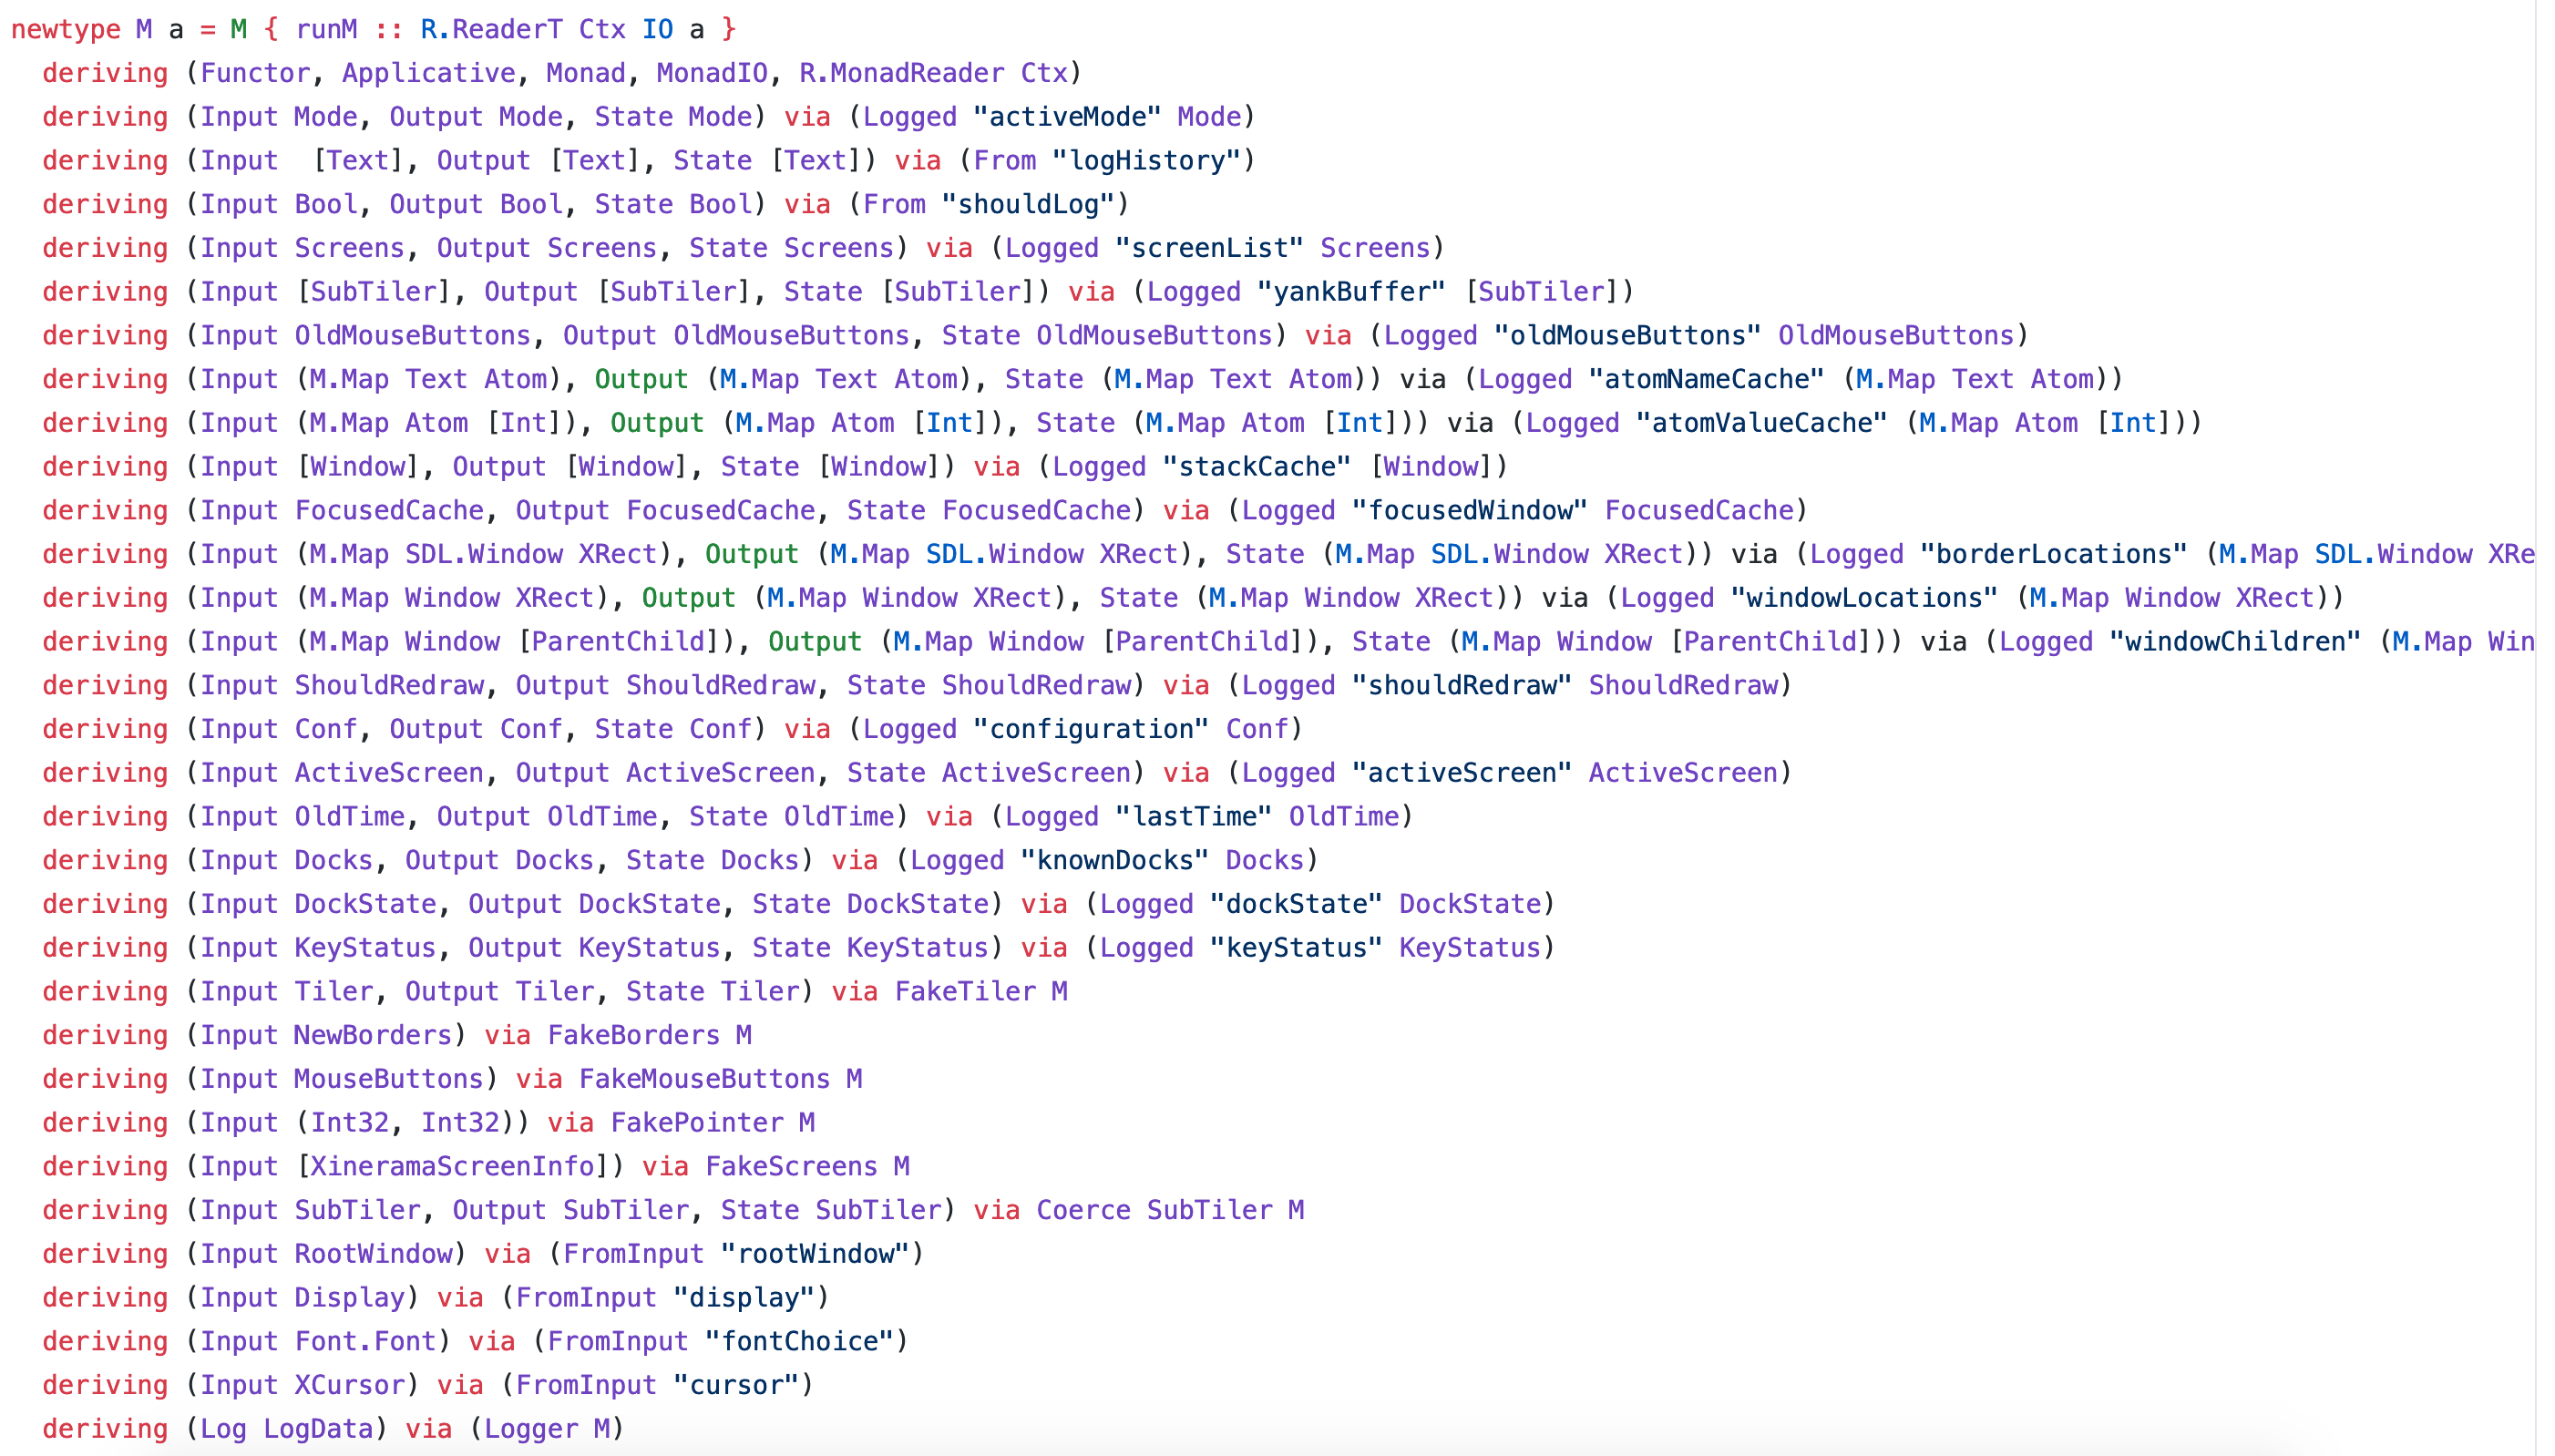
\includegraphics[scale=0.5,width=\linewidth]{figures/deriving-via-example.png}
    \caption{Example of deriving information in Haskell. source:\url{https://github.com/jhgarner/Xest-Window-Manager/blob/3741b35a69eb2cf8cd7320e186fd40134d1c1a56/src/Base/DoAll.hs}}
    \label{fig:deriving-via-example}
\end{figure}

This DSL would change the activity of theory development in the following way 
\begin{itemize}
    \item Save the human effort put in reproducing standard knowledge by internalizing this knowledge in the generation algorithm.
    \item Maintain a level of flexibility towards changing design decisions by understanding how they affect the generated definitions.
    \item Increase the usability of library definitions by reducing the amount of design decisions baked into them. 
\end{itemize}  

%The definitions we use in our development are based on universal algebra abstractions. Universal algebra abstracts over algebraic structures and their related constructions and provides the meta theory that explains how the generation algorithms should work. A theory presentation in universal algebra has three components \verb|(S,F,E)|; a sort \verb|S|, a list of function symbols along with their types \verb|F|, and a list of axioms (equations) that describe properties of the function symbols \verb|E|. If we can abstract over the details of theory presentations to extract this information, we are able to generate the constructions defined by universal algebra, like morphisms, product algebras, term languages, and others. 

In this work, we attempt to answer the following research questions 
\begin{enumerate}
    \item[RQ1] Can the uniformity provided by universal algebra be captured by a meta program that generates parts of an algebra library?
    \item[RQ2] What design decisions need to be abstracted from and which ones can be reintroduced after the generation of new?
    \item[RQ3] Which information need to be provided by the developer and which ones can be generated? 
    \item[RQ4] What are the preconditions for generating this new information? 
    \item[RQ5] How would this affect the activity of library building?
    \item[RQ6] Can these generation algorithms be extended beyond uni-sorted first-order theories, the ones that universal algebra captures? 
\end{enumerate}

\section{Contributions}
\begin{itemize}
    \item Highlight the redundancy in algebra libraries 
    \item Compile a list of structures that can be generated from theory presentations
    \item Generate some of these constructions in Tog, a small implementation of a dependently typed language, in the style of Agda, Coq and Lean. 
    \item Export this implementation to Agda 
    \item Test our framework on a library of over $200$ theories implemented using the combinators defined in~\cite{carette2018building}. 
\end{itemize}  

\section{Broader Context}
\label{sec:broader_context}
There are different ways of organizing knowledge within a formal system. Our work contributes to building a large math library organized as a theory graph in the heart of a tetrapodal structure. Theory graphs, explained in details in Section~\ref{sec:background:theorygraph}, capture the structure of mathematical knowledge by enabling the description of relationships between the different pieces using morphisms. Using them, we can express facts like `a group is a monoid` and that `monoid and additive monoid are isomorphic`. 

The nodes of a theory graph can be any kind of theories. Ideally, they would be biform theories~\cite{biformCICM2018}, as they connect axiomatic theories (used by theorem provers), and algorithmic theories (used by computer algebra systems) using meaning formulas. That way it facilitates communication between reasoning and computational systems; it becomes possible to reason about algorithmic theories, and to use results of computer algebra systems in theorem provers. In this work we only look at axiomatic theories. 

Morphisms are meaning preservation maps. The simplest form of a morphism is inclusion. Morphisms are used to transfer results from one theory to another. So, a morphism between \lstmath{Monoid} and \lstmath{AdditiveMonoid} that describes they are isomorphic, allows us to transfer results between them. 

In~\cite{carette2020bigMath}, the authors argue that modern mathematics is organized as a tetrapod with knowledge organization being at its center. We are working towards a library organized as a theory graph of biform theories that serves as this center. Different aspects of the tetrapod will be consumers and producers of knowledge in this library. This implies that the size of this library would be huge, and that using generative approach to support its building would be a great asset. 

We support the building of this library by providing combinators to define the library theories and algorithms to compute related constructions



\begin{comment}  
These algebraic concepts are very important in mathematics and computer science that they are a main component in libraries of almost every mechanized system\ednote{add citations on research of algebra library development}. We consider the \lstmath{Monoid} structure for our running example. a \lstmath{Monoid} consists of a carrier over which there is an associative binary operation that has a unit. If we look at algebra textbooks, we find that~\cite{mckenzie1987algebras} defines it as 
\begin{quote}%[mathescape]
A monoid is an algebra $A = \langle \cdot^A, e^A \rangle$ such that 
$\langle A, \cdot^A \rangle$ is a semigroup and \\
$a \cdot^A e^A = e^A \cdot^A a = a$ for all $a \in A$.
\end{quote}
In~\cite{jacobson1985basic}, it is defined as 


Algebra text books would follow the definition of an algebraic structure with the definitions of some of its related constructions, like subalgebras, homomorphisms, term languages, quotients, etc. The scope of the book might determine which ones are included. \cite{jacobson1985basic} provides the following definition of monoid homomorphism 

and proceeds to talk about \lstmath{Group} homomorphism depending on the human ability to infer it from its given definition of \lstmath{Monoid}. 

Moving to formal systems, We find that they also do not agree on one definition of the theory \lstmath{Monoid}. Figure~\ref{fig:mon-diff-lang} shows its definition in $5$ different languages. 
\begin{figure}
\footnotesize
\begin{tabular}{p{6.3cm} p{7cm}}
\underline{Haskell}
\begin{minted}[mathescape]{haskell}
class Semigroup a => 
      Monoid a 
 where 
  mempty :: a 
  mappend :: a -> a -> a 
  mappend = (<>) 
  mconcat :: [a] -> a 
  mconcat = 
   foldr mappend mempty 
\end{minted} 
\underline{Lean}
\begin{leancode}
class monoid (M : Type u)
 extends semigroup M, 
         has_one M :=
  (one_mul : ~$\forall$~ a : M, 
           1 * a = a) 
  (mul_one : ~$\forall$~ a : M, 
           a * 1 = a)   
\end{leancode} 
% [mathescape=true, escape_inside=~~]
\underline{Coq}
\begin{minted}[mathescape=true, escapeinside=~~]{coq}
class Monoid {A : type}
 (dot : A ~$\to$~ A ~$\to$~ A)
 (one : A) : Prop := {
  dot_assoc : 
   forall x y z : A, 
   (dot x (dot y z)) = 
   dot (dot x y) z
  unit_left : forall x, 
   dot one x = x 
  unit_right : forall x, 
   dot x one = x              
}
~$\text{\textit{Alternative Definition:}}$~
Record monoid := {
 dom : Type; 
 op : dom -> dom -> dom 
  where "x * y" := op x y; 
 id : dom where "1" := id; 
 assoc : forall x y z, 
  x * (y * z) = (x * y) * z; 
 left_neutral : forall x,   
  1 * x = x; 
 right_neutal : forall x,
  x * 1 = x; 
}
\end{minted} 
&
\underline{Agda}
\begin{agdacode}
record Monoid c ~$\ell$~ : 
   Set (suc (c ~$\sqcup$~ ~$\ell$~)) where 
 infixl 7 _~$\bullet$~_
 infix 4 _~$\approx$~_
 field 
  Carrier : Set c 
  _~$\approx$~_ : Rel Carrier ~$\ell$~ 
  _~$\bullet$~_ : Op~$_2$~ Carrier 
  isMonoid : IsMonoid _~$\approx$~_ _~$\bullet$~_ ~$\varepsilon$~ 
  
record IsMonid (~$\bullet$~ : Op~$_2$~) (~$\varepsilon$~ : A) 
 : Set (a ~$\sqcup$~ ~$\ell$~) where 
  field 
   isSemiring : IsSemiring ~$\bullet$~ 
   identity : Identity ~$\varepsilon$~ 
       
   open IsSemigroup isSemigroup public 
   
   identity~$^l$~ : LeftIdentity ~$\varepsilon$~ ~$\bullet$~ 
   identity~$^l$~ = proj~$_1$~ identity 
   identity~$^r$~ : Rightdentity ~$\varepsilon$~ ~$\bullet$~ 
   identity~$^r$~ = proj~$_2$~ identity        
\end{agdacode}       
\underline{MMT}
\begin{minted}[mathescape=true, escapeinside=~~]{mmt} 
theory Semigroup : ?NatDed = 
 u : sort 
 comp : tm u ~$\to$~ tm u ~$\to$~ tm u 
  # 1 * 2 prec 40
 assoc : ~$\vdash$~ ~$\forall$~ [x, y, z]
  (x * y) * z = x * (y * z)    
 assocLeftToRight : 
  {x,y,z} ~$\vdash$~ (x * y) * z 
          = x * (y * z) 
  = [x,y,z] 
   allE (allE (allE assoc x) y) z
 assocRightToLeft : 
  {x,y,z} ~$\vdash$~  x * (y * z) 
           = (x * y) * z 
  = [x,y,z] sym assocLR 
theory Monoid : ?NatDed 
 includes ?Semigroup 
 unit : tm u # e 
 unit_axiom : ~$\vdash$~ ~$\forall$~ [x] = x * e = x       
\end{minted}      
\end{tabular}  

\caption{Representation of \lstinline|Monoid| theory in different languages.}
\label{fig:mon-diff-lang}
\end{figure}
For now, we imagine a definition of \lstmath{Monoid} in a simple language as follows 
\begin{lstlisting}[mathescape]
theory Monoid { 
A : type 
e : A
op : A $\to$ A $\to$ A
lunit : $\cdots$
runit : $\cdots$
assoc : $\cdots$ 
}
\end{lstlisting}        
The homomorphism of \lstmath{Monoid} in the same language is 
\begin{lstlisting}[mathescape]
theory MonoidHom { 
M1, M2 : Monoid  
hom : M1.A $\to$ M2.A 
pres-e : $\cdots$
pres-op : $\cdots$
}
\end{lstlisting}
The components of the homomorphism are $2$ instances of \lstmath{Monoid} theory, a mapping from the carrier of one instance to the other, and preservation axiom for every function symbols that follow the pattern 
\begin{lstlisting}[mathescape]
hom (op$_1$ x$_1$ .. x$_n$) = op$_2$ (hom x$_1$) .. (hom x$_n$)
\end{lstlisting}
Notice how all these components can be derived from the definition of \lstmath{Monoid}. 

Another commonly used algebraic structure is \lstmath{Group}. In order to use it in a formal system, one needs to define it along with all its related definitions that they need, like \lstmath{Group} homomorphism which follows the same pattern described above. This observation lead us to the question 
\end{comment}



\begin{comment}
Notice how all the 
~\cite{mckenzie1987algebras} is 
\begin{quote}%[mathescape]
A monoid is an algebra $A = \langle \cdot^A, e^A \rangle$ such that 
$\langle A, \cdot^A \rangle$ is a semigroup and \\
$a \cdot^A e^A = e^A \cdot^A a = a$ for all $a \in A$.
\end{quote}
Note how \lstmath{Monoid} is defined in terms of a smaller theory \lstmath{Semigroup}. While inthe definition given is  

In this case, \lstmath{Monoid} is defined in terms of its components. Both ways of defining \lstmath{Monoid} are useful and humans can switch between these definition without overhead. Depending on the task intended by the user, they might have a preference of one over the other. 
\end{comment}


%We focus our attention to algebra libraries which formalizes core concepts in mathematics and computer science. Algebra libraries contain axiomatic formalization of algebraic structures. Those structures describe classes of algebras. For example the algebras $(\mathbb{N},+,0)$ and $(Strings,++,\varepsilon)$ have similar behavior that is captured with the algebraic structure \lstmath{Monoid}. Defining and proofing properties of a structure is enough to define/prove it to all its models (all the algebras it describes). In the process of working with algebraic structures, one need some constructions related to them, like homomorphism, subalgebras, term algebras, etc. 
